\chapter{Introduction}

\section{Petri nets}

\subsection{Overview}

Petri nets are a graphical and mathematical modeling tool used to describe and analyze the behavior of concurrent systems.
They were introduced by the German researcher Carl Adam Petri in his doctoral dissertation \cite{petri1962}
and have since been applied in a variety of fields such as computer science, engineering, and biology.
A concise summary of the theory of Petri nets, its properties, analysis and applications can be found in \cite{murata1989}.

A Petri net is a bipartite digraph consisting of a set of places, transitions and arcs.
There are two types of nodes, namely places and transitions.
Places represent the state of the system, while transitions represent events or actions that can occur.
Arcs connect places to transitions or transitions to places.
There can be no arcs between places nor transitions, thus preserving the bipartite property.

Places may hold zero or more tokens.
Tokens are used to represent the presence or absence of entities in the system, such as resources, data, or processes.
In the most simple class of Petri nets, tokens do not carry any information and they are indistinguishable from one another.
The number of tokens at a place or the simple presence of a token is what conveys meaning in the net.
Tokens are consumed and produced as transitions fire, giving the impression that they move through the arcs.

In the conventional graphical representation, places are depicted using circles, while transitions are depicted as rectangles.
Tokens are represented as black dots inside of the places, as seen in \ref{fig:petri-net-example}.

\begin{figure}[H]
    \centering
    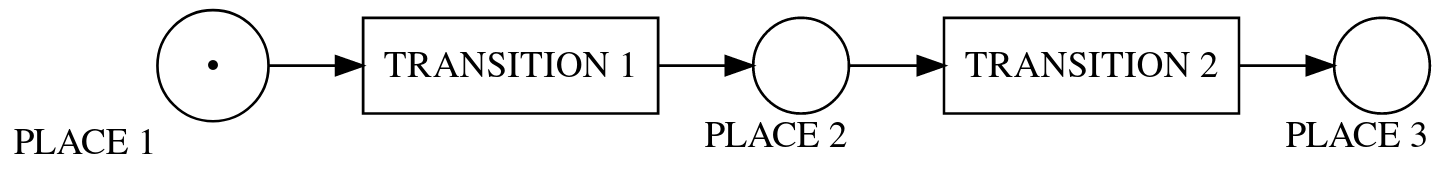
\includegraphics[scale=0.25]{petri-net-example.png}
    \caption{Example of a Petri net. \uppercase{PLACE 1} contains a token.}
    \label{fig:petri-net-example}
\end{figure}

When a transition fires, it consumes tokens from its input places and produces tokens in its output places, reflecting a change in the state of the system.
The firing of a transition is enabled when there are sufficient tokens in its input places.
In \ref{fig:petri-net-transition-firing-example}, we can see how successive firings happen.

\begin{figure}[H]
    \centering
    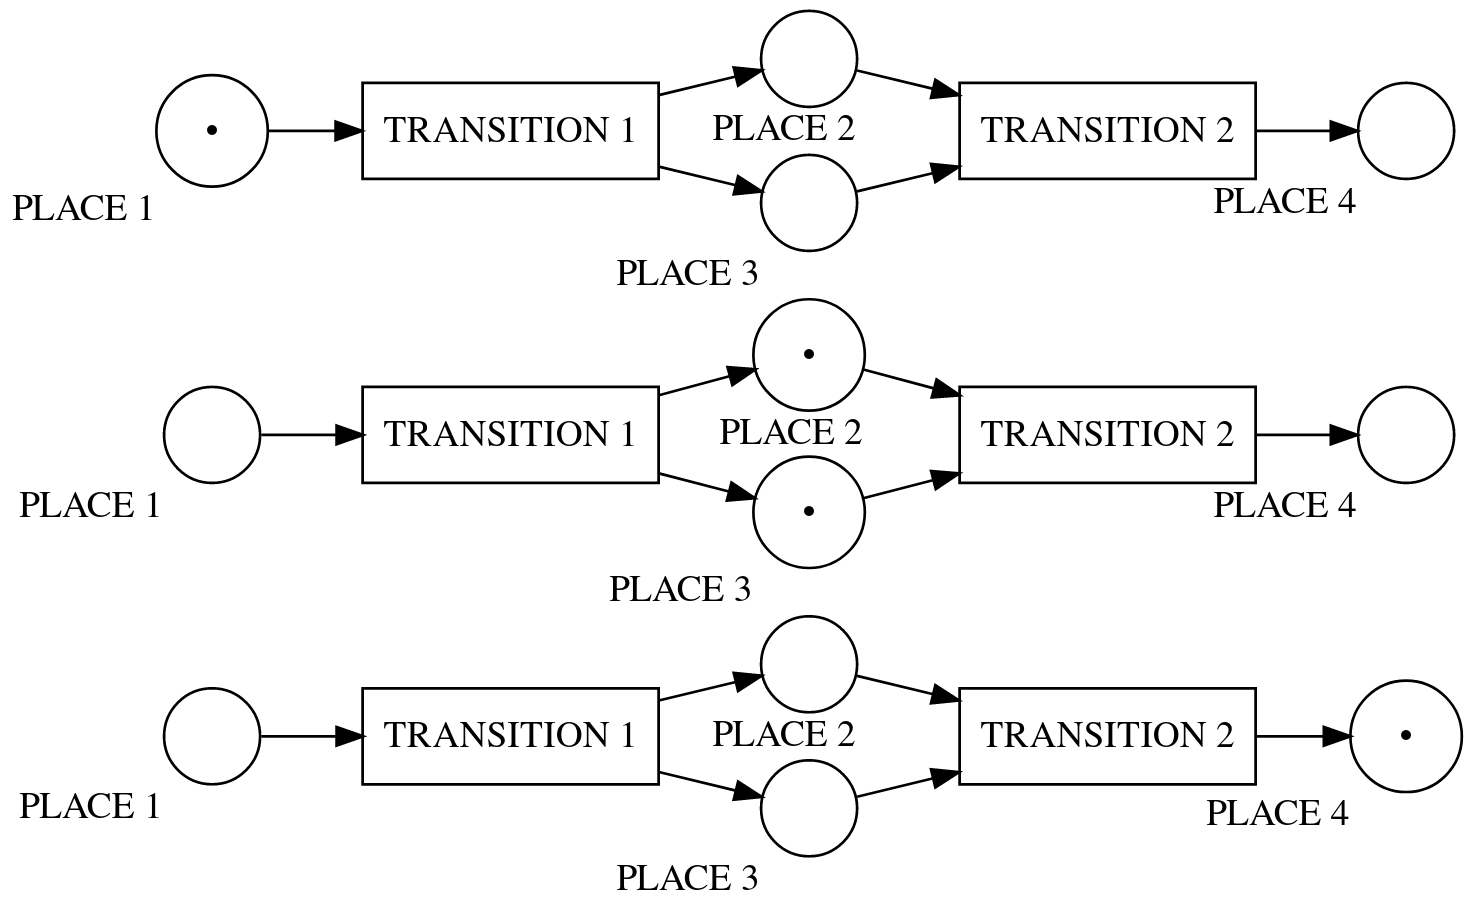
\includegraphics[scale=0.25]{petri-net-transition-firing-example.png}
    \caption{Example of transition firing. First, transition 1 fires, then transition 2 fires.}
    \label{fig:petri-net-transition-firing-example}
\end{figure}

The firing of enabled transitions is not deterministic, i.e., they fire randomly as long as they are enabled.
A disabled transition is considered \textbf{dead} if there is no reachable state in the system that can lead to the transition being enabled.
If all the transitions in the net are dead, then the net is considered \textbf{dead} too.
This state is analogous to the deadlock of a computer program.

Petri nets can be used to model and analyze a wide range of systems, from simple systems with a few components to complex systems with many interacting components.
They can be used to detect potential problems in a system, optimize system performance and design and implement systems more effectively.

In particular, Petri nets can be used to detect deadlocks in source code by modeling the input program as a Petri net
and then analyzing the structure of the resulting net.
It will be shown that this approach is formally sound and
practicably amenable to source code written in the Rust programming language.

\subsection{Formal mathematical model}

\section{The Rust programming language}

\section{Deadlocks}

\section{Lost signals}

\section{Compiler arquitecture}

\section{Model checking}

\bigskip